\chapter{滴定}\label{ch:g11:titration}

补铁剂包装盒上标明，每片含铁 \qty{80}{mg}
（以亚铁离子计）。这一说法是否属实？
一位化学家将药片研碎，用酸溶解，并
从一根长滴定管中逐滴加入紫色的高锰酸钾溶液。每一滴都立即褪色，
因为高锰酸根离子被亚铁离子消耗；直到最后一滴，
使溶液呈淡粉色，且不再褪去。
此时滴入的体积即为铁的物质的量。本章要把
一个反应转化为一次测量。

\begin{recall}
氧化剂得到电子，还原剂失去电子；高锰酸根离子
按下式氧化亚铁离子：
\ce{MnO4^- + 8H+ + 5Fe^{2+} -> Mn^{2+} + 5Fe^{3+} + 4H2O}
（见\cref{ch:g11:redox}）。物质的量浓度与稀释
（见\cref{ch:g10:concentration-and-dilution}）；进度表与
限量反应物（见\cref{ch:g10:reaction-progress-table}）。
\end{recall}

\begin{omfigure}
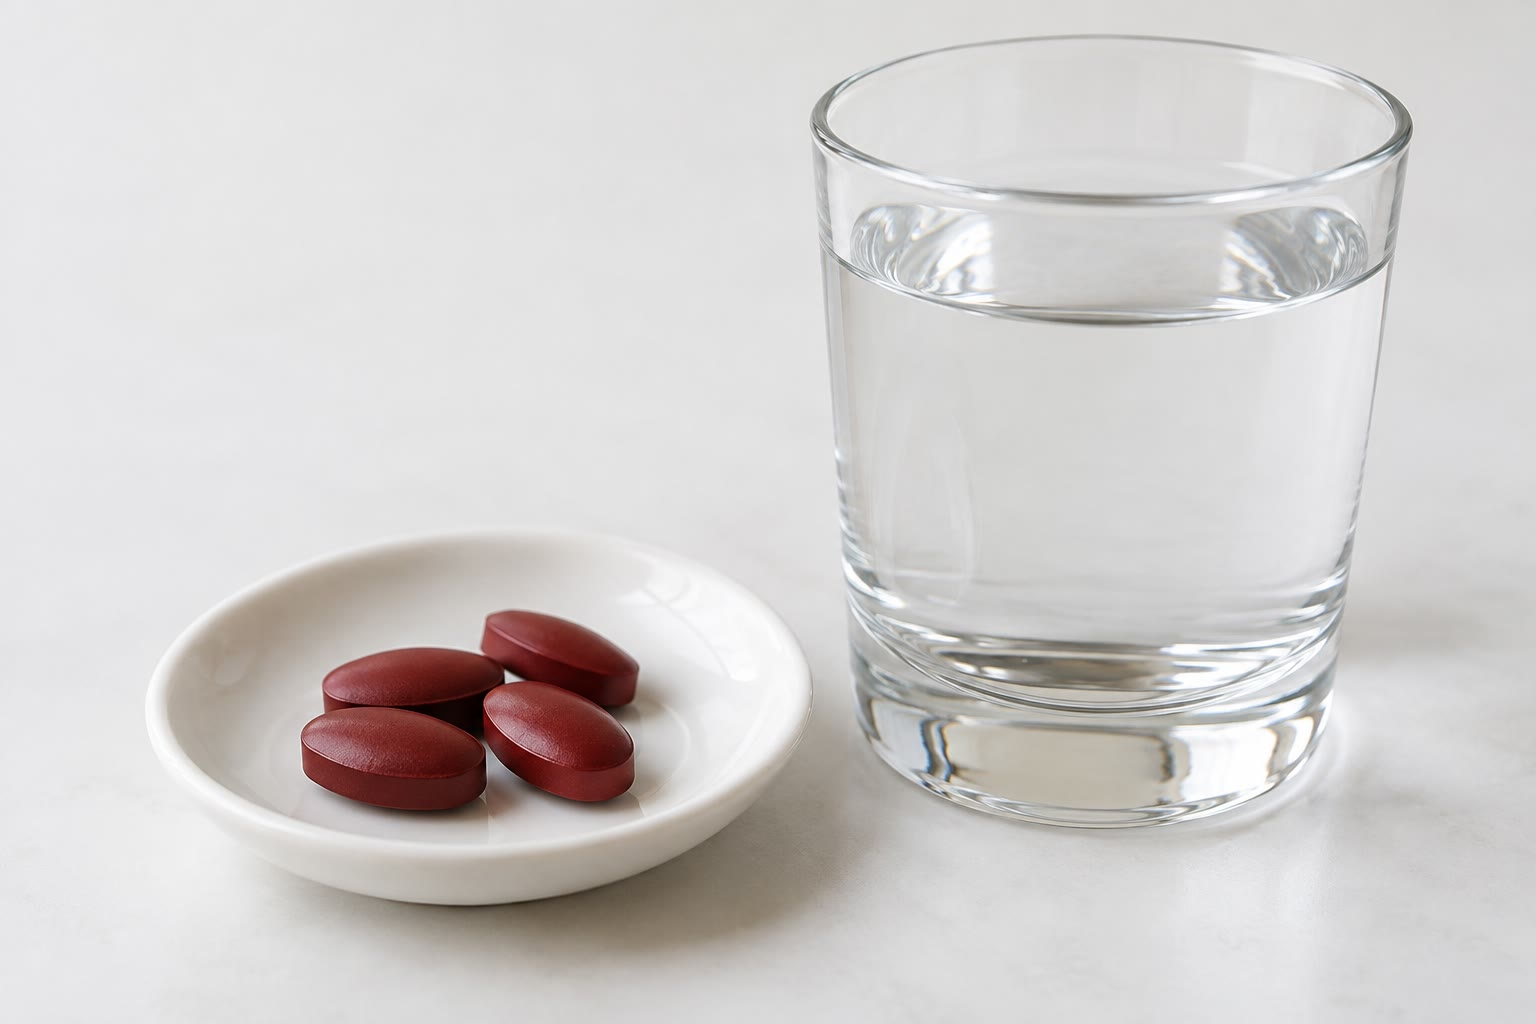
\includegraphics[width=0.45\linewidth]{images/book1/ai/g11-iron-tablets.jpg}

{\small 铁补充剂药片：每片究竟含铁多少？}
\end{omfigure}

\section{滴定操作}

\begin{definition}[滴定、滴定剂、被滴定溶液]\label{def:g11:titration:titration}
\emph{滴定}\index{滴定}是测定某已溶解物质的量的方法，
即让其与浓度准确已知的另一物质反应。已知浓度的溶液，
由滴定管加入，即为\emph{滴定剂}\index{滴定剂}；
含有待测物质并置于锥形瓶中的溶液，
即为\emph{被滴定
溶液}\index{被滴定溶液}。
\end{definition}

\begin{proposition}[滴定反应须满足的条件]\label{prop:g11:titration:conditions}
用于滴定的反应须满足以下条件：完全，即其中一种反应物被完全消耗；
迅速，即每一滴都能立即反应；
专一，即滴定剂不与瓶中其他物质发生反应。
\end{proposition}

\begin{proof}
若反应未进行完全，或落后于滴加速度，
或滴定剂被他处消耗，则所加体积
便不能再反映被滴定物质的量。
\end{proof}

\begin{omfigure}
\begin{tikzpicture}[font=\small, scale=0.62]
  \pic[transform shape] at (0,0) {stand={5.8}{1.8}};
  \pic[transform shape] at (1.8,0.68) {stirrer};
  \pic[transform shape] at (1.8,0.68) {erlenmeyer={0.25}{yellow!12}};
  \pic[transform shape] at (1.8,2.98) {burette={0.75}{violet!55}};
  \draw[omProp, thick, <-] (2.15,6.9) -- (4.2,7.4) node[right, text=black,
    align=left] {滴定管：滴定剂 \\（高锰酸钾）};
  \draw[omProp, thick, <-] (2.55,1.4) -- (4.2,1.9) node[right, text=black,
    align=left] {锥形瓶：被滴定 \\溶液（亚铁离子、酸）};
  \draw[omProp, thick, <-] (3.0,0.4) -- (4.2,0.3) node[right, text=black]
    {磁力搅拌器};
\end{tikzpicture}

{\small 滴定装置：滴定管固定在支架上，将滴定剂
加入正在搅拌的被滴定溶液中。}
\end{omfigure}

\section{滴定终点}

\begin{definition}[滴定终点、等当点体积]\label{def:g11:titration:equivalence}
\emph{滴定终点}\index{滴定终点}是滴定中所加滴定剂与
被滴定物质恰好按方程式的比例反应、两者均被耗尽的时刻。
此时所滴入滴定剂的体积
即为\emph{等当点体积}\index{等当点体积}，$V_E$。
\end{definition}

\begin{proposition}[滴定终点的关系]\label{prop:g11:titration:relation}
对于滴定反应 $a\,\ce{A} + b\,\ce{B} \longrightarrow$ 生成物，A 被滴定（物质的量
为 $n_A$），以浓度为 $c_B$ 的滴定剂 B 滴定，在滴定终点时有
\[
  \frac{n_A}{a} = \frac{c_B\, V_E}{b} .
\]
\end{proposition}

\begin{proof}
滴定终点时，混合物恰好按化学计量比反应
（见\cref{ch:g10:reaction-progress-table}）：A、B 的初始物质的量分别为 $n_A$
和 $c_B V_E$，二者同时耗尽，故 $n_A / a = c_B V_E / b$。
\end{proof}

\begin{omfigure}
\begin{tikzpicture}
\begin{axis}[width=0.72\linewidth, height=5.6cm, xmin=0, xmax=20,
    ymin=0, ymax=16, xlabel={加入滴定剂的体积（\si{mL}）},
    ylabel={物质的量（$\num{e-4}$ \si{mol}）}, axis lines*=left, ymajorgrids,
    grid style={gray!20}, tick label style={font=\small},
    label style={font=\small}, legend style={font=\small, at={(0.98,0.97)},
    anchor=north east, draw=none}, legend cell align=left]
  \addplot[very thick, orange!70!black, domain=0:14.3] {14.3 - x};
  \addplot[very thick, violet, domain=14.3:20] {0.2*(x - 14.3)};
  \addplot[very thick, violet, domain=0:14.3, forget plot] {0};
  \legend{\ce{Fe^{2+}} 剩余于锥形瓶中，\ce{MnO4^-} 过量}
  \addplot[dashed, black!60] coordinates {(14.3,0) (14.3,7)};
  \node[font=\small, anchor=west] at (axis cs:14.5,6.5) {$V_E = \qty{14.3}{mL}$};
\end{axis}
\end{tikzpicture}

{\small 用浓度为 \qty{0.0200}{mol/L} 的高锰酸钾溶液滴定亚铁离子：
亚铁离子恰好在等当点体积时耗尽；此后，
高锰酸根离子不再被消耗，而是逐渐积累。}
\end{omfigure}

\section{通过颜色变化确定滴定终点}


\begin{proposition}[观察滴定终点]\label{prop:g11:titration:colour}
滴定中若有一种物质带有颜色，则滴定终点
表现为锥形瓶中颜色的变化：滴定剂的颜色出现
并在滴定剂过量时持续存在；或是
被滴定物质的颜色在其耗尽时消失。
\end{proposition}

\begin{proof}
滴定终点之前，每个落入锥形瓶的滴定剂离子
立即被消耗；滴定终点之后，则会残留。带色物质
因此仅在滴定终点的一侧存在于锥形瓶中。
\end{proof}

\begin{example}[高锰酸根，自身即指示剂]\label{ex:g11:titration:permanganate}
高锰酸根离子 \ce{MnO4^-} 呈深紫色，而它生成的锰离子
\ce{Mn^{2+}} 几乎无色；亚铁离子只使溶液
带淡黄色。滴定终点之前，每一滴紫色液滴
落入时都会立即褪色；第一滴未褪色的
液滴标志着滴定终点：锥形瓶变为淡粉色，并保持不变。
\end{example}

\begin{omfigure}
\begin{tikzpicture}[font=\small]
  \pic at (0,0) {erlenmeyer={0.3}{yellow!14}};
  \pic at (3.2,0) {erlenmeyer={0.3}{magenta!10}};
  \pic at (6.4,0) {erlenmeyer={0.3}{violet!45}};
  \node[align=center, anchor=north] at (0,-0.15) {滴定终点之前：\\
    淡黄色，每滴 \\ 均被褪色};
  \node[align=center, anchor=north] at (3.2,-0.15) {滴定终点时：\\
    淡粉色，且 \\ 持续存在};
  \node[align=center, anchor=north] at (6.4,-0.15) {滴定终点之后：\\
    紫色（高锰酸根 \\ 过量）};
\end{tikzpicture}

{\small 高锰酸钾滴定亚铁离子时锥形瓶的状态：滴定终点前、
滴定终点时及之后。等当点体积应读取于第一次持续出现的
淡粉色时。}
\end{omfigure}

\begin{example}[维生素 C 与碘]\label{ex:g11:titration:vitamin-c}
% ledger: aw:C, aw:H, aw:O
维生素 C，即抗坏血酸 \ce{C6H8O6}（$M = \qty{176.0}{g/mol}$），是一种
还原剂；碘 \ce{I2} 可将其氧化：
\[
  \ce{C6H8O6 + I2 -> C6H6O6 + 2H+ + 2I-} .
\]
\qty{10.0}{mL} 橙汁，加入少量淀粉，用
浓度为 \qty{5.00e-3}{mol/L} 的碘溶液滴定。滴定终点之前，碘
被消耗；过量的第一滴碘液使淀粉变为深蓝色。若
$V_E = \qty{5.70}{mL}$，则橙汁中
维生素 C 的物质的量为 $n = \num{5.00e-3} \times \num{5.70e-3} = \qty{2.85e-5}{mol}$，
即 \qty{10.0}{mL} 中含 \qty{5.0}{mg}，浓度为 \qty{0.50}{g/L}。
\end{example}

\section{计算未知浓度}

\begin{method}[由滴定计算浓度]\label{met:g11:titration:computing}
\begin{enumerate}
  \item 写出滴定反应的配平方程式，并读出
        系数 $a$（被滴定物质）与 $b$（滴定剂）。
  \item 在滴定管上读出 $V_E$，并计算所加入
        滴定剂的物质的量 $n_B = c_B V_E$。
  \item 滴定终点时，$n_A = \dfrac{a}{b}\, c_B V_E$。
  \item 除以被滴定溶液的体积：$c_A = n_A / V_A$。若试样
        在滴定前经过稀释，则乘以稀释倍数。
\end{enumerate}
\end{method}

\begin{example}[一种亚铁离子溶液]\label{ex:g11:titration:iron}
\qty{20.0}{mL} 酸化的亚铁离子溶液，恰好需
$V_E = \qty{12.6}{mL}$ 浓度为 \qty{0.0200}{mol/L} 的高锰酸钾溶液。此处
$a = 5$（\ce{Fe^{2+}}）、$b = 1$（\ce{MnO4^-}）：
$n(\ce{MnO4^-}) = 0.0200 \times 0.0126 = \qty{2.52e-4}{mol}$，于是
$n(\ce{Fe^{2+}}) = 5 \times \num{2.52e-4} = \qty{1.26e-3}{mol}$，且
$c(\ce{Fe^{2+}}) = \num{1.26e-3} / 0.0200 = \qty{0.0630}{mol/L}$。
\end{example}

\section{滴定作为一种测量}

\begin{inthelab}[读取滴定管]
滴定管先用滴定剂润洗、注满，并排除尖嘴中的
气泡。在弯月面底部读取液面刻度，读数时视线
与液面等高，滴定前后均如此；所加体积为
两次读数之差。刻度每 \qty{0.1}{mL} 一格，读数可
估读至 \qty{0.05}{mL}。接近滴定终点时，滴定剂逐滴加入
并不断摇动或搅拌锥形瓶。
\end{inthelab}

\begin{omfigure}
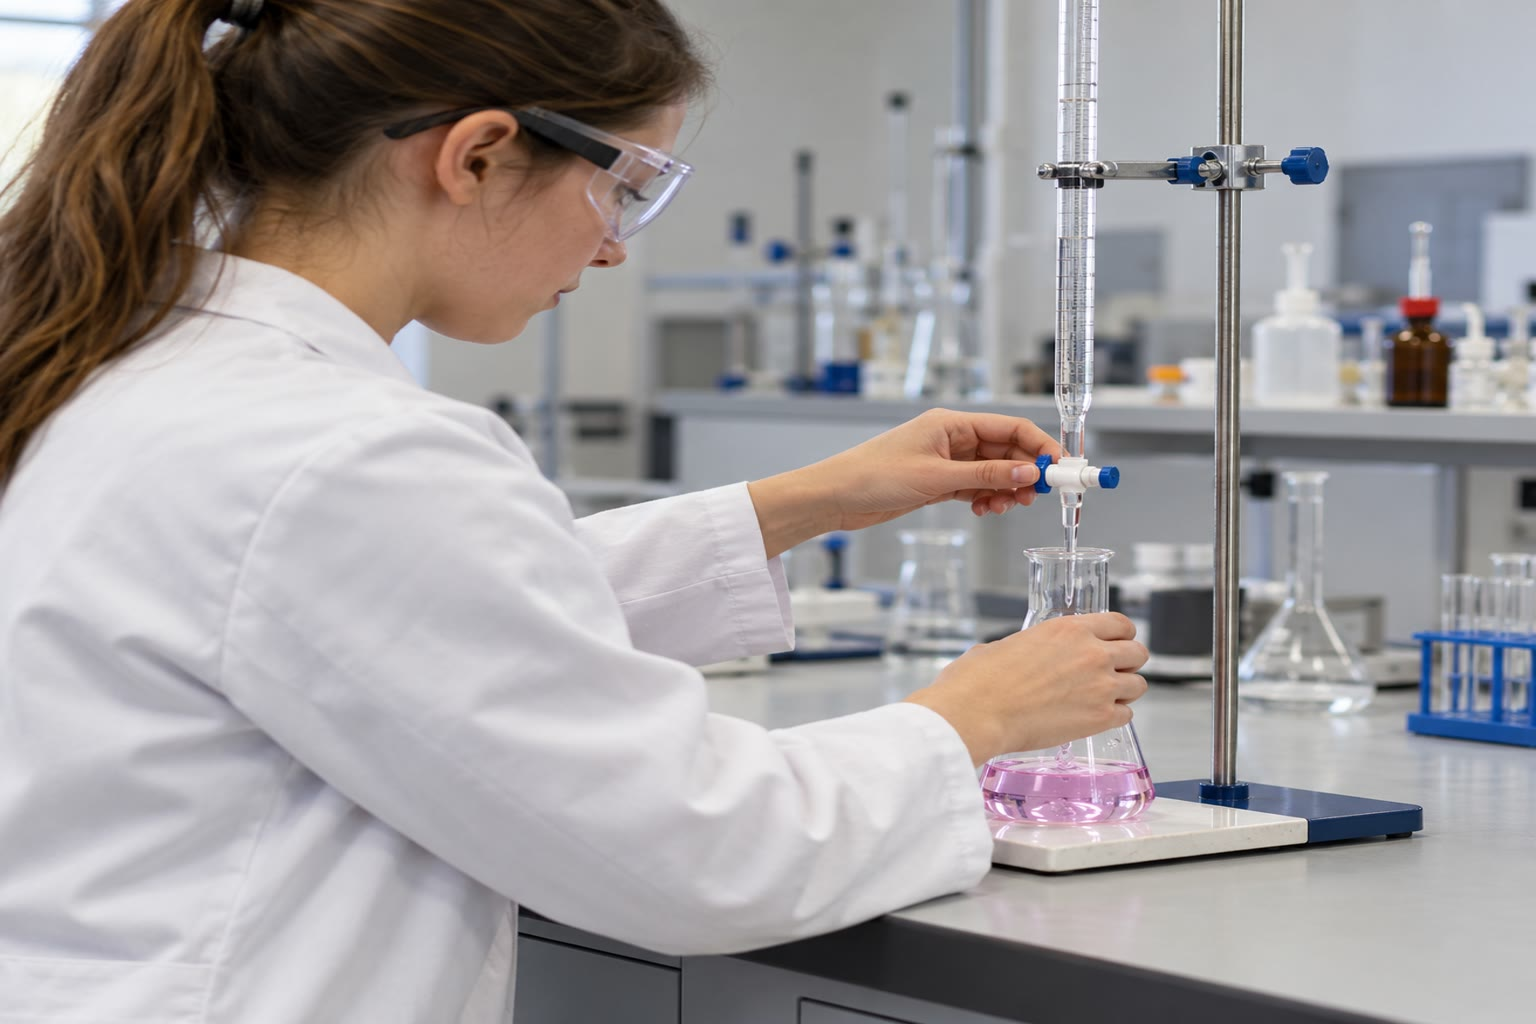
\includegraphics[width=0.48\linewidth]{images/book1/ai/g11-titration-bench.jpg}

{\small 滴定进行中：滴定管、铁架台与锥形瓶放在
白色瓷砖上。}
\end{omfigure}

\begin{remark}[滴定的精度有多高？]\label{rem:g11:titration:precision}
滴定管每次读数可能有约 \qty{0.05}{mL} 的误差，所加体积
为两次读数之差，误差至多为 \qty{0.1}{mL}。
对于 $V_E = \qty{14.3}{mL}$，相对误差约为 $0.1 / 14.3 \approx
\qty{0.7}{\percent}$。$V_E$ 越大，相对误差越小，
这也解释了为什么要选择滴定剂浓度，使等当点体积
为 10 至 \qty{20}{mL}，并配合 \qty{25}{mL} 的滴定管。
滴定须反复进行，直至两次结果之差
约在 \qty{0.1}{mL} 之内。测量不确定度的更精细处理，
见于本科一年级分册。
\end{remark}

\begin{safety}{\ghs[0.7cm]{GHS03}\ghs[0.7cm]{GHS05}\ghs[0.7cm]{GHS07}\ghs[0.7cm]{GHS08}\ghs[0.7cm]{GHS09}}
% ledger: ghs:KMnO4, ghs:I2
固体高锰酸钾是一种氧化剂，可助燃，
具有腐蚀性和有害性；其稀溶液会使皮肤和衣物染成棕色。碘溶液
有害。须佩戴护目镜和手套；废液须收集，
切勿倒入水槽。
\end{safety}

\section{练习}


\begin{exercise}[$\star$]\label{exo:g11:titration:1}
在滴定中，滴定剂是什么？被滴定溶液是什么？
滴定终点时发生什么？
\end{exercise}

\begin{exercise}[$\star$]\label{exo:g11:titration:2}
求 \qty{12.5}{mL} 浓度为 \qty{0.0200}{mol/L} 的
溶液中所含高锰酸根离子的物质的量。
\end{exercise}

\begin{exercise}[$\star$]\label{exo:g11:titration:3}
根据物质的量随所加体积变化的图，
读出等当点体积。
开始时锥形瓶中铁(II)的物质的量是多少？
\end{exercise}

\begin{exercise}[$\star$]\label{exo:g11:titration:4}
用高锰酸钾滴定时为什么不需要指示剂？
\end{exercise}

\begin{exercise}[$\star$]\label{exo:g11:titration:5}
用高锰酸钾滴定铁(II)时，在滴定终点，
铁(II)的物质的量与所加高锰酸根离子的物质的量之比为多少？
为什么？
\end{exercise}

\begin{exercise}[$\star\star$]\label{exo:g11:titration:6}
\qty{10.0}{mL} 酸化的铁(II)溶液需用 \qty{8.40}{mL}
浓度为 \qty{0.0200}{mol/L} 的高锰酸钾溶液。求
铁(II)的物质的量浓度，再求其质量浓度。
\end{exercise}

\begin{exercise}[$\star\star$]\label{exo:g11:titration:7}
将一片维生素 C 药片溶解，配成 \qty{100.0}{mL} 溶液。
取其中 \qty{10.0}{mL}，加淀粉，需 \qty{11.4}{mL} 浓度为
\qty{0.0100}{mol/L} 的碘溶液。求该药片所含维生素 C 的质量。
\end{exercise}

\begin{exercise}[$\star\star$]\label{exo:g11:titration:8}
某反应进行完全，但需要几分钟。为什么它不能直接用于
以颜色变化判断终点的滴定？
\end{exercise}

\begin{exercise}[$\star\star$]\label{exo:g11:titration:9}
观察三个锥形瓶。某同学停止滴定时，锥形瓶中的紫色
与第三个一样深。她的等当点体积偏大还是偏小？
她在接近滴定终点时本应如何操作？
\end{exercise}

\begin{exercise}[$\star\star$]\label{exo:g11:titration:10}
将浓铁(II)溶液先稀释十倍，然后取稀释后的
\qty{10.0}{mL} 溶液，需用 \qty{13.0}{mL} 浓度为
\qty{0.0200}{mol/L} 的高锰酸钾溶液。
求浓溶液的浓度。
\end{exercise}

\begin{exercise}[$\star\star$]\label{exo:g11:titration:11}
% ledger: aw:Fe
本章例题中的铁(II)溶液，
其浓度为 $c = \qty{0.0630}{mol/L}$。求 \qty{1.00}{L} 该溶液
中所含铁的质量。
\end{exercise}

\begin{exercise}[$\star\star\star$]\label{exo:g11:titration:12}
某次滴定得 $V_E = \qty{7.2}{mL}$。估算由滴定管读数
引起的相对误差，并与 $V_E = \qty{14.3}{mL}$ 的情形相比较，提出
两种增大等当点体积的方法。
\end{exercise}

\begin{exercise}[$\star\star\star$]\label{exo:g11:titration:13}
在酸性条件下用高锰酸钾滴定过氧化氢：
\[
  \ce{2MnO4^- + 5H2O2 + 6H+ -> 2Mn^{2+} + 5O2 + 8H2O} .
\]
某消毒液稀释十倍后，取其中 \qty{10.0}{mL}，
需用 \qty{17.6}{mL} 浓度为 \qty{0.0200}{mol/L} 的高锰酸钾溶液。
求消毒液中过氧化氢的物质的量浓度，
再求其质量浓度（\ce{H2O2}：\qty{34.0}{g/mol}）。
\end{exercise}

\begin{exercise}[$\star\star\star$]\label{exo:g11:titration:14}
某铁片应含约 \qty{1.4e-3}{mol} 铁(II)。
若要使等当点体积接近
\qty{15}{mL}，并使用 \qty{25}{mL} 滴定管，高锰酸根离子的浓度应为多少？
若所用溶液浓度增大十倍，会出现什么问题？
\end{exercise}

\begin{exercise}[$\star\star\star$]\label{exo:g11:titration:15}
滴定反应方程式表明，\ce{8H+} 对应每个 \ce{MnO4^-}。对于等当点体积为
\qty{14.3}{mL}、浓度为 \qty{0.0200}{mol/L} 的高锰酸钾溶液，
被消耗的氢离子的物质的量是多少？
取 \qty{10}{mL} 含氢离子浓度为 \qty{1.0}{mol/L} 的酸，是否足够？
为什么必须酸化锥形瓶？
\end{exercise}

\section{问题：铁片的标示是否属实？}

\begin{problem}[{周末问题——一种铁补充剂声称
每片含 80 mg 铁：滴定结果是否相符？}]
\label{pb:g11:titration:1}
% ledger: aw:Fe, aw:S, aw:O, const:NA
某铁补充剂包装盒上标明，每片含 \qty{80}{mg} 铁（以铁(II)计）。
将一片药片研碎后溶于约 \qty{50}{mL} 稀硫酸中，
再用 \qty{0.0200}{mol/L} 的高锰酸钾溶液滴定。
淡粉色持续不褪时，$V_E = \qty{14.3}{mL}$。

\medskip
\noindent\textbf{第一部分——反应。}
\begin{enumerate}
  \item 指出涉及的两个氧化还原电对，
        哪种物质是氧化剂，哪种是还原剂？
  \item 写出两个半反应式。
  \item 将两个半反应式合并为滴定反应的方程式，
        并检查其电荷是否配平。
  \item 为什么要用酸溶解药片？
  \item 说明该反应满足滴定的条件，
        并解释如何观察到滴定终点。
\end{enumerate}

\medskip
\noindent\textbf{第二部分——滴定。}
\begin{enumerate}[resume]
  \item 高锰酸钾溶液应盛放在哪种玻璃仪器中？
        其体积如何读取？
  \item 滴定终点前，锥形瓶中溶液呈什么颜色？
        每滴一滴溶液为何会褪色？
  \item 计算滴定至终点时所加入高锰酸钾的物质的量。
\end{enumerate}

\medskip
\noindent\textbf{第三部分——铁。}
\begin{enumerate}[resume]
  \item 推算药片中亚铁离子的物质的量。
  \item 计算其质量，单位为毫克。
  \item 与标签比较：相对差是多少？
  \item 所加入的体积可能有 \qty{0.1}{mL} 的偏差，
        则铁的质量可能偏差多少毫克？标签是否得到证实？
\end{enumerate}

\medskip
\noindent\textbf{第四部分——若干片药片。}
\begin{enumerate}[resume]
  \item 另外两片药片分别给出 $V_E = \qty{14.1}{mL}$ 和
        \qty{14.4}{mL}，计算它们所含铁的质量。
  \item 计算三片药片结果的平均值。
  \item 三个结果之间的差异超过了滴定管的误差，
        这说明药片有什么问题？
  \item 若改用 \qty{0.100}{mol/L} 的高锰酸钾溶液，会是更好的选择吗？
        请说明理由。
  \item 许多补充剂还含有维生素 C，它是一种还原剂。
        它会对滴定以及测得的铁的质量产生什么影响？
  \item 铁以硫酸亚铁 \ce{FeSO4} 的形式存在。
        一片药片中含有多少质量的硫酸亚铁？
  \item 这相当于多少个亚铁离子？
  \item 给出最终答案：
        一片药片中含有多少质量的铁？
\end{enumerate}
\end{problem}
